Per l'esecuzione dell'esperienza è stato utilizzato il seguente apparato sperimentale:
\begin{itemize}
	\item Guida ottica
	\item Piattaforma rotante graduata
	\item Laser
	\item Prisma di vetro di apertura $\alpha=45^{\circ}$
	\item Schermo
	\item Sostegni
\end{itemize}

\begin{table}[H]
	\centering
	\begin{tabular}{|c|c|}
		\hline
		\textbf{Strumenti di misura} & \textbf{Risoluzione} \\
		\hline
		Piattaforma rotante graduata & $1^{\circ}$ \\
		\hline
	\end{tabular}
	\caption{Risoluzione degli strumenti di misura utilizzati}
	\label{tab:}
\end{table}

\begin{figure}[H]
	\centering
	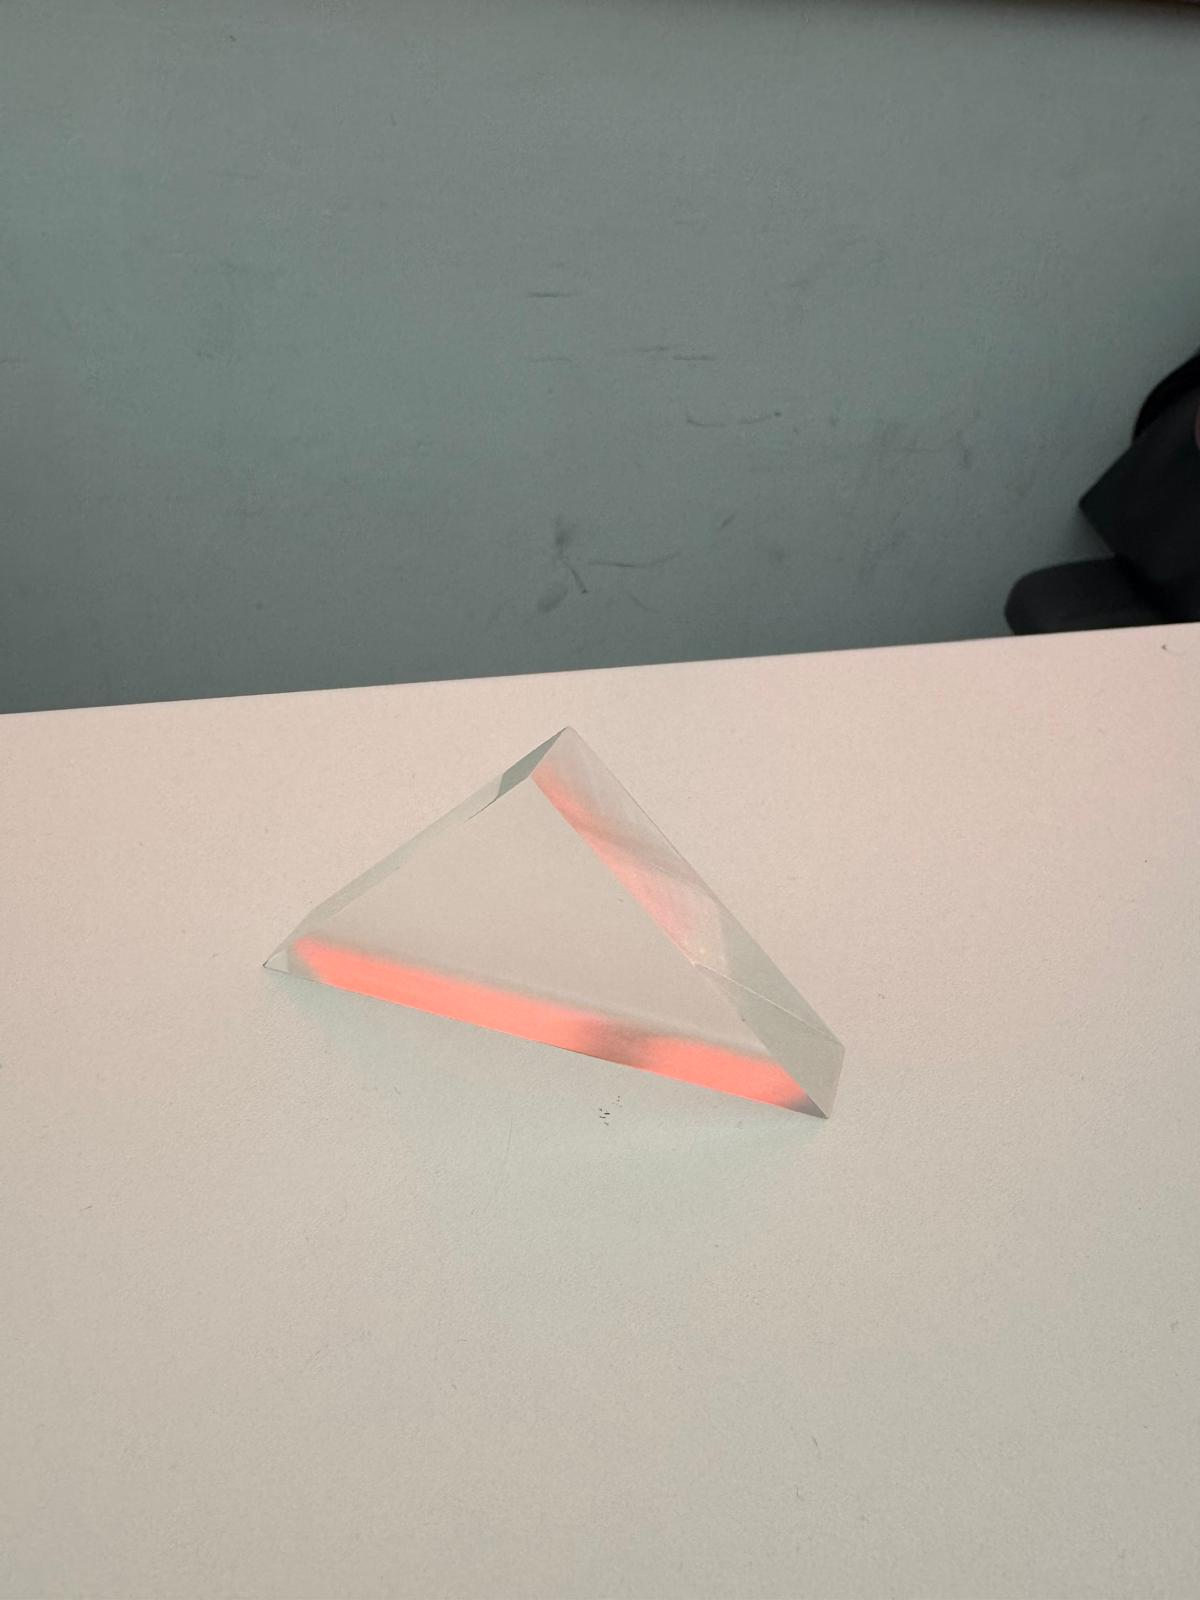
\includegraphics[width=0.55\textwidth]{./figures/prisma}
	\caption{Prisma utilizzato per l'esperimento.}
\end{figure}

\begin{figure}[H]
	\centering
	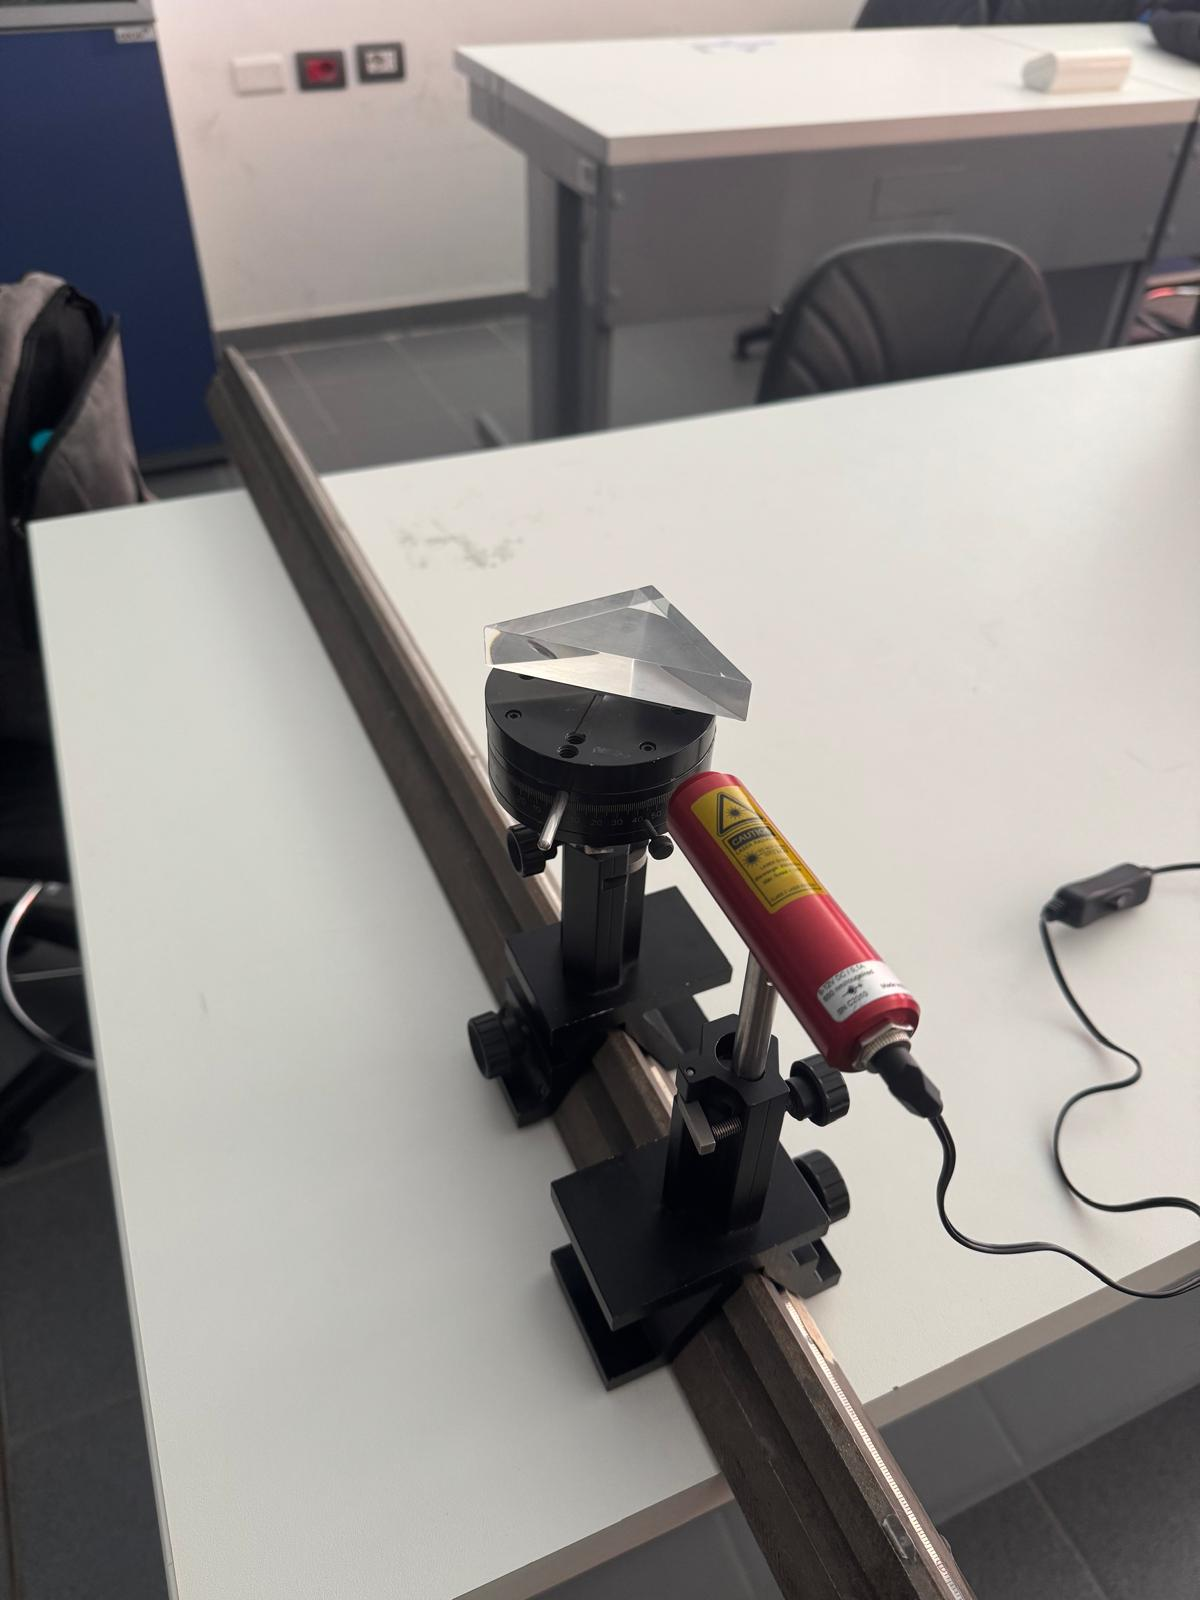
\includegraphics[width=0.55\textwidth]{./figures/apparato}
	\caption{Strumenti assemblati per l'esecuzione dell'esperienza.}
\end{figure}

\begin{figure}[H]
	\centering
	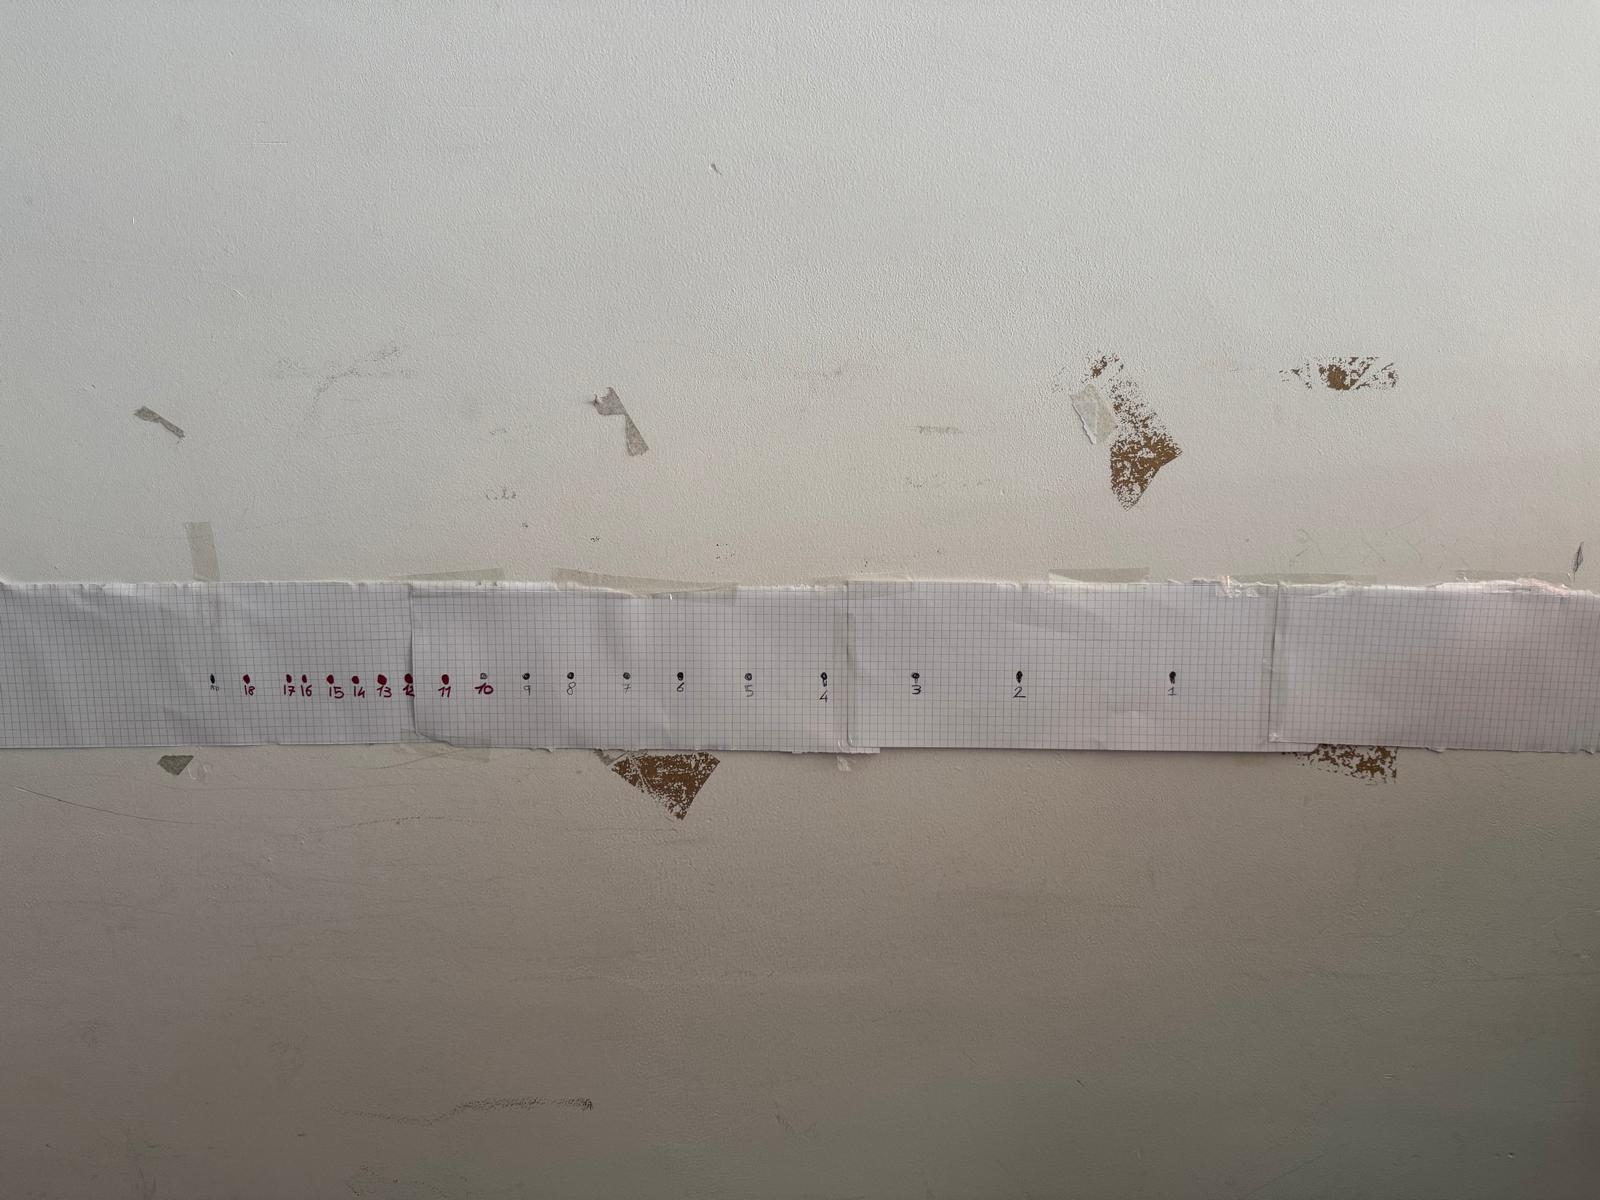
\includegraphics[width=0.55\textwidth]{./figures/nastro}
	\caption{Schermo su cui sono stati indicati i punti di intersezione del raggio laser in corrispondenza dei quali sono stati misurati gli angoli $\theta_i$ e $\theta_i'$.}
\end{figure}